%
% Qualificacao_Doutorado.tex (LateX)
% 
% Objetivo: Arquivo principal do relatório de qualificação de doutorado.
% baseado em um template para a geração de documentos em LaTeX.
% 
% Versão 1.0
% 
% Site: http://www.dirackslounge.online
% 
% Programador: 
%		(1.4) - Lauro César Araujo 
%			Template, distribuição e manutenção
%		(1.5) - Rodolfo A. C. Neves (Dirack) 07/10/2019 
%			Modificações e utilização neste relatório
% 
% Email: rodolfo_profissional@hotmail.com
% 
% Licença (Versão modificada): GPL-3.0 <https://www.gnu.org/licenses/gpl-3.0.txt>.
%
% Licença (Versão original): LaTeX Project Public License (LPPL - 1.3) <http://www.latex-project.org/lppl.txt>
%
% Documentação extra: <http://abntex2.googlecode.com/>

\documentclass[
	% -- opções da classe memoir --
	12pt,				% tamanho da fonte
	openright,			% capítulos começam em pág ímpar (insere página vazia caso preciso)
	oneside,			% para impressão em verso e anverso. Oposto a oneside
	a4paper,			% tamanho do papel. 
	% -- opções da classe abntex2 --
	%chapter=TITLE,		% títulos de capítulos convertidos em letras maiúsculas
	%section=TITLE,		% títulos de seções convertidos em letras maiúsculas
	%subsection=TITLE,	% títulos de subseções convertidos em letras maiúsculas
	%subsubsection=TITLE,% títulos de subsubseções convertidos em letras maiúsculas
	% -- opções do pacote babel --
	english,			% idioma adicional para hifenização
%	french,				% idioma adicional para hifenização
%	spanish,			% idioma adicional para hifenização
	brazil				% o último idioma é o principal do documento
	]{abntex2}

\usepackage{multirow}
\usepackage{amsmath}
\usepackage{tocloft}
\usepackage{cmap}			% Mapear caracteres especiais no PDF
\usepackage{lmodern}			% Usa a fonte Latin Modern			
\usepackage[T1]{fontenc}		% Seleção de códigos de fonte.
\usepackage[utf8]{inputenc}		% Determina a codificação utiizada (conversão automática dos acentos)
\usepackage{makeidx}            	% Cria o indice
\usepackage{amssymb,amsfonts,amsmath,wasysym}
\usepackage{lastpage}			% Usado pela Ficha catalográfica
\usepackage{indentfirst}		% Indenta o primeiro parágrafo de cada seção.
\usepackage{nomencl} 			% Lista de simbolos
\usepackage{color}			% Controle das cores
\usepackage{graphicx}			% Inclusão de gráficos
\usepackage{microtype} 			% para melhorias de justificação
\usepackage{subfig}
\usepackage{float} 			% Colocar a figura no local certo
\usepackage{scalefnt} 			% Pacote da redimensionar a fonte de tabelas, figuras e equações.
\usepackage{placeins}
\allowdisplaybreaks
\usepackage{kantlipsum}
\usepackage{pdfpages}
\usepackage{titlesec}
\usepackage[brazilian,hyperpageref]{backref}	 % Paginas com as citações na bibl
\usepackage[alf]{abntex2cite}			 % Citações padrão ABNT
\usepackage{tensor}
\usepackage{setspace}
\usepackage{caption}

\renewcommand{\figurename}{Figura-}
\usepackage[figurename=Figura]{caption}

\renewcommand{\chapnumfont}{\bfseries}
\renewcommand{\ABNTEXfontereduzida}{\mdseries\footnotesize}
\renewcommand{\ABNTEXchapterfontsize}{\bfseries \normalsize}
\renewcommand{\ABNTEXsectionfontsize}{\normalsize}
\addto{\captionsbrazil}{\renewcommand{\contentsname}{\textbf{SUMÁRIO}}}
\addto{\captionsbrazil}{\renewcommand{\bibname}{\bfseries \textbf{REFERÊNCIAS}\selectfont}}
\renewcommand{\apendicesname}{\bfseries \selectfont  APÊNDICES}
\renewcommand{\apendicename}{\bfseries\selectfont APÊNDICE}
\renewcommand{\anexosname}{\bfseries ANEXOS}

\renewcommand*{\backrefalt}[4]{
	\ifcase #1
	
	\or
	
	\else

	\fi}

%% Informações básicas da CAPA
\instituicao{
  Universidade Federal do Pará -- UFPA
  \par
  Instituto de Geociências
  \par
  Programa de Pós-Graduação em Geofísica}
\titulo{INTERPOLAÇÃO DE DADOS SÍSMICOS NO DOMÍNIO ERC UTILIZANDO AS APROXIMAÇÕES DE TEMPO DE TRÂNSITO SRC PADÉ}

\autor{Rodolfo André Cardoso Neves}
\local{Belém-Pará}
\data{2019}

\orientador{Prof. Dr. João Carlos Ribeiro Cruz}
\coorientador{}

\preambulo{Relatório apresentado ao Programa de Pós-Graduação em Geofísica do Instituto de Geociências 
da Universidade Federal
do Pará, em cumprimento às exigências para obtenção do grau de Doutor em Geofísica.}

\definecolor{blue}{RGB}{41,5,195}
\definecolor{black2}{RGB}{39,64,139}

%% Configurações padrão do PDF
\hypersetup{
		backref=true,
		pagebackref=true,
		bookmarks=true,         		% show bookmarks bar?
		pdftitle={\imprimirtitulo}, 
		pdfauthor={\imprimirautor},
    	pdfsubject={\imprimirpreambulo},
		pdfkeywords={PALAVRAS}{CHAVES}{abnt}{abntex}{abntex2},
	    pdfproducer={LaTeX with abnTeX2}, 		% producer of the document
	    pdfcreator={\imprimirautor},
    	colorlinks=true,       				% false: boxed links; true: colored links
    	linkcolor=black,          			% color of internal links
    	citecolor=black,        			% color of links to bibliography
    	linkcolor=black,          			% color of internal links
    	citecolor=black,        			% color of links to bibliography
    	filecolor=black,      				% color of file links
		urlcolor=black,
		bookmarksdepth=4
}

% Indentação do parágrafo
\setlength{\parindent}{1.3cm}

% Espaçamento entre parágrafos
\setlength{\parskip}{0.2cm}

% Espaçamento entre linhas
\OnehalfSpacing	

% compilar indice
\makeindex

% Compilar lista de abreviaturas e siglas
\makenomenclature

\renewcommand{\sin}{\mathrm{sen}}
\newcommand{\disp}{\displaystyle}
\newcommand{\mbf}{\mathbf}

\hyphenation{geo-fí-si-co}
\hyphenation{MCSEM}

\captionsetup{labelsep=period,font=small,justification=justified,labelfont=md,format=plain,labelsep=endash}

\renewcommand{\imprimircapa}{
\begin{capa}
	\begin{figure}[!t]
		\begin{center}
			
\includegraphics[scale=0.3]{images/Logo_UFPA2.pdf}
		\end{center} 
	\end{figure}
			\begin{center}
				{\ABNTEXchapterfont\bfseries{UNIVERSIDADE FEDERAL DO PARÁ \\ INSTITUTO DE GEOCIÊNCIAS \\ PROGRAMA DE PÓS-GRADUAÇÃO EM GEOFÍSICA} }
		\end{center}

\center

\vspace*{1cm}
{\ABNTEXchapterfont\bfseries\large\MakeUppercase{\imprimirautor}}\\
\vspace*{2cm}
{\ABNTEXchapterfont\bfseries\large\imprimirtitulo}\\
\vspace*{2cm}{\ABNTEXchapterfont\bfseries\large{RELATÓRIO DE QUALIFICAÇÃO DE DOUTORADO}}
\vspace*{\fill}\\
{\large\MakeUppercase{\imprimirlocal}}
\par
{\large\imprimirdata}
\vspace*{1cm}
\end{capa}
}


\makeatletter
\renewcommand{\folhaderostocontent}{
\begin{center}
	\vspace*{1cm}
	{\ABNTEXchapterfont\bfseries\large\MakeUppercase{\imprimirautor}}\\
	\vspace*{\fill}\vspace*{\fill}
	{\ABNTEXchapterfont\bfseries\large\imprimirtitulo}\\
	 \vspace{\baselineskip}
	{\ABNTEXchapterfont\bfseries\large{RELATÓRIO DE QUALIFICAÇÃO DE DOUTORADO}}
	\vspace{\baselineskip}
	\vspace{\baselineskip}
	\vspace*{\fill}
	\abntex@ifnotempty{\imprimirpreambulo}{
	\hspace{5cm}
	\begin{minipage}{10cm}
	\SingleSpacing
	\imprimirpreambulo\\ \\
	{\imprimirorientadorRotulo~Prof. Dr. João Carlos Ribeiro Cruz}\\
	\end{minipage}
	\vspace*{\fill}
	}
	\abntex@ifnotempty{\imprimircoorientador}{
	{\large\imprimircoorientadorRotulo~\imprimircoorientador}
	}
	\vspace*{\fill}
	{\large\imprimirlocal}
	\par
	{\large\imprimirdata}
	\vspace*{1cm}
\end{center}

}

\makeatother

\begin{document}

\imprimircapa

\imprimirfolhaderosto*

\begin{dedicatoria}
   \vspace*{\fill}
   \vspace*{13cm}
   \centering
   \noindent
   \begin{flushright} Dedico este trabalho \`a minha fam\'ilia.
   \end{flushright}
     \vspace*{\fill}
\end{dedicatoria}

\begin{agradecimentos}[\fontsize{12pt}{\baselineskip}\textbf{AGRADECIMENTOS}]
\vspace*{1.5cm}

Ao Prof. Dr. João Carlos pela orientação desta tese, e pela proposta do tema. Além
do suporte e paciência em responder as minhas dúvidas, e das sugestões inteligentes na solução de problemas
que foram aparecendo no caminho.

Agradeço ao professor Sergey Fomel, que apesar de não conhecer pessoalmente, produziu trabalhos
que inspiraram o tema, e disponibilizou gratuitamente
vários
dos programas aqui utilizados.

Agradeço à minha mãe Regina de Nazaré,
à minha irmã Rebeca Cristina, às minhas sobrinhas Ágatha e Anadora, 
e ao meu pai Ricardo Neves, por todo apoio e dedicação
durante a árdua caminhada para a realização deste sonho!

E agradeço à amizade de amigos que conquistei durante o curso de Geofísica, e que de forma direta ou indireta
me ajudaram na realização do trabalho:
Leonardo Reis, Hugo Souza, Diogo Rezende, Antônio Rizimar e Raphael Di Carlo.

\end{agradecimentos}

\begin{epigrafe}
    \vspace*{\fill}
	\begin{flushright}
		\textit{``Todas as coisas excelentes são tão difíceis quanto raras''. \\
		(Baruch Spinoza)}
	\end{flushright}
\end{epigrafe}

\begin{resumo}[\fontsize{12pt}{\baselineskip}\textbf{RESUMO}]
\OnehalfSpacing
O método do elemento de reflexão comum (ERC) é uma alternativa para os métodos
usuais de empilhamento ou migração para a seção de afastamento nulo. Porém, diferente do empilhamento 
convencional, em que os pares são dispostos em famílias de ponto médio comum (PMC) de maneira simétrica ao 
PMC central, a disposição dos pares fonte-receptor é assimétricamente disposta em famílias ERC. 
Haverá pontos sobre a curva ERC onde não existem dados adiquiridos e será necessário realizar a interpolação. 
Assim, o empilhamento ERC pode ser realizado, mesmo a partir de uma 
aquisição sísmica convencional e de dados organizados em famílias PMC.
 \vspace{\onelineskip} 
 \noindent
 \par Palavras-chave: Empilhamento Superfície de Reflexão Comum (SRC). Aproximações não hiperbólicas do tempo de trânsito SRC. 
 Interpolação Elemento de Reflexão Comum (ERC). 
\end{resumo}

\begin{resumo}[\fontsize{12pt}{\baselineskip}\textbf{ABSTRACT}]
\OnehalfSpacing
The common reflection element method (CRE) is an alternative to usual stacking and migration methods 
in zero offset section domain. Besides convencional stacking, wich source receiver pairs are simetricaly distributed into common 
midpoint gathers (CMP) in the neighboorhood of a central CMP, in CRE gathers the disposition of 
source-receiver pairs is assimetric. There are points in CRE curve where there is no data and interpolation is crucial. 
So, CRE gather interpolation can be used to provide information data 
and allow CRE stacking, despite convencional CMP gather as input.
\vspace{\onelineskip} 
\noindent 
\par Keywords: Padé approximants. Common Reflection Surface (CRS) stacking. Non Hyperbolic CRS.
Common Reflection Element (CRE) interpolation.
\end{resumo}

\renewcommand{\listfigurename}{\fontsize{12pt}{\baselineskip}\textbf{LISTA DE ILUSTRAÇÕES}}
\pdfbookmark[0]{\listfigurename}{lof}
\listoffigures*

\cleardoublepage

\tableofcontents*

\cleardoublepage
 
\mainmatter

%% Inclusão dos capítulos ao documento principal
%
% cre.tex (LateX)
% 
% Objetivo: Capítulo sobre o método CRE do relatório de qualificação de doutorado.
% 
% Versão 1.0
% 
% Site: http://www.dirackslounge.online
% 
% Programador: Rodolfo A. C. Neves (Dirack) 07/10/2019
% 
% Email: rodolfo_profissional@hotmail.com
% 
% Licença: GPL-3.0 <https://www.gnu.org/licenses/gpl-3.0.txt>.

\chapter{EMPILHAMENTO ELEMENTO DE REFLEXÃO COMUM (ERC)}
\label{cap2:cre}

O método empilhamento Elemento de Reflexão Comum (ERC) é uma alternativa para os métodos de empilhamento PMC ou
migração para a seção de afastamento nulo. Não requer conhecimento do modelo geral em subsuperfície, apenas
o conhecimento da velocidade próxima a superfície é necessário a priori.
O método ERC é baseado somente em considerações cinemáticas em 2D e não é
um processo que preserva as amplitudes.
A principal vantagem do método ERC em comparação com o empilhamento PMC convencional
é que este proporciona a seção empilhada e parâmetros importantes para a construção do macromodelo de 
velocidades que pode inclusive variar lateralmente \cite{cre}.

As principais características do método ERC são:
\begin{enumerate}
 \item[(a)] A construção da seção de afastamento nulo a partir de um conjunto de seções de afastamento constante
com apenas uma estimativa da velocidade próxima da superfície.

 \item[(b)] A determinação dos parâmetros $(R_{NIP},\beta_0)$ para as reflexões de afastamento nulo na seção empilhada.
Estes atributos podem ser utilizados com técnicas de inversão para estimar o macromodelo de velocidades.
\end{enumerate}

Os parâmetros $R_{NIP}$ e $\beta_0$ 
são atributos específicos de uma frente de onda hipotética atribuídos a cada evento de reflexão
primária de afastamento nulo: O raio de curvatura $R_{NIP}$ e o ângulo de emergência $\beta_0$. Esta onda hipotética é
a onda NIP \cite{hubral}.

A idéia principal do método ERC é usar a fórmula do tempo de trânsito ERC no modelo auxiliar para
encontrar a frente de onda NIP que melhor se ajusta aos dados, dado um intervalo
de busca para os parâmetros $R_{NIP}$ e $\beta_0$,
Este processo é semelhante a análise sobretempo normal convencional, todavia enquanto esta análise é feita no
domínio PMC, o método ERC é feito no domínio ERC construído durante o processo. Os parâmetros otimizados $R_{NIP}$ e $\beta_0$
são especificados a partir da análise de coerência nos dados \cite{cre}.

As coordenadas das curvas ERC, mesmo sem o conhecimento da curvatura do refletor em subsuperfície, são definidas
a partir dos parâmetros $R_{NIP}$ e $\beta_0$, obtidos através de um processo de otimização, 
para cada PMC central $m_0$ na seção de afastamento nulo. A Equação que descreve a trajetória ERC no plano $m, h$ \cite{cre}:

\begin{equation}
 \label{eq:2.1}
 m= m_0 + \frac{1}{2\alpha} (1-\sqrt{1+4\alpha^2h^2})
\end{equation}

Onde $\alpha$ é um parâmetro de assimetria que desenpenha um papel importante na seleção de pares fonte-receptor para os quais
os correspondentes raios de reflexão incidem no mesmo ponto sobre o refletor \cite{tygel}. E é dado por:

\begin{equation}
\label{eq:2.2}
 \alpha=\frac{\sin{\beta_0}}{R_{NIP}}
\end{equation}

Os traços sísmicos com as coordenadas $m, h$ dadas pela Equação \ref{eq:2.1} formam uma família ERC.
O método ERC também possui uma aproximação de tempo de trânsito de
reflexão \cite{cre}:

\begin{multline}
\label{eq:2.3}
t(m,h)= \left( \tau_0-\frac{2R_{NIP}}{v_0} \right) 
+\frac{R_{NIP}}{v_0}\sqrt{1-2\alpha(m-m_0+h)+\frac{(m-m_0+h)^2}{R_{NIP}^2}} \\
\end{multline}

Onde $t(m,h)$ é o tempo de trânsito de reflexão no domínio ERC para o PMC $m$ e o meio afastamento $h$.
$v_0$ é a velocidade próxima da superfície, $\tau_0$ é o tempo de trânsito de afastamento nulo e 
$R_{NIP}$ e $\alpha$ são os parâmetros otimizados associados a um PMC central $m_0$.

A Equação \ref{eq:2.3} é utilizada para o empilhamento no domínio ERC. As amostras nas famílias ERC 
que estão sobre esta curva de tempo de trânsito são empilhadas e atribuídas ao PMC central $m_0$ na seção empilhada.
Ao realizar este processo para todos os $m_0$'s da malha obtemos a imagem na seção empilhada ERC.

\begin{figure}[H]
\caption{Representação esquemática de um arranjo ERC para um refletor circular de raio $R$ e profundidade
mínima $D$: A família ERC é formada pelos pares $s_i$-$r_i$ (fonte-receptor) que possuem o mesmo ponto de
reflexão em subsuperfície (ponto $NIP$). A família ERC pode ser entendida a partir de uma fonte pontual explosiva
no ponto $NIP$, que ao ser ativada forma uma frente de onda $NIP$ que atinge a superfície em um PMC central 
$m_0$ com raio de curvatura $R_{NIP}$ e ângulo de incidência $\beta_0$.}
\begin{center}
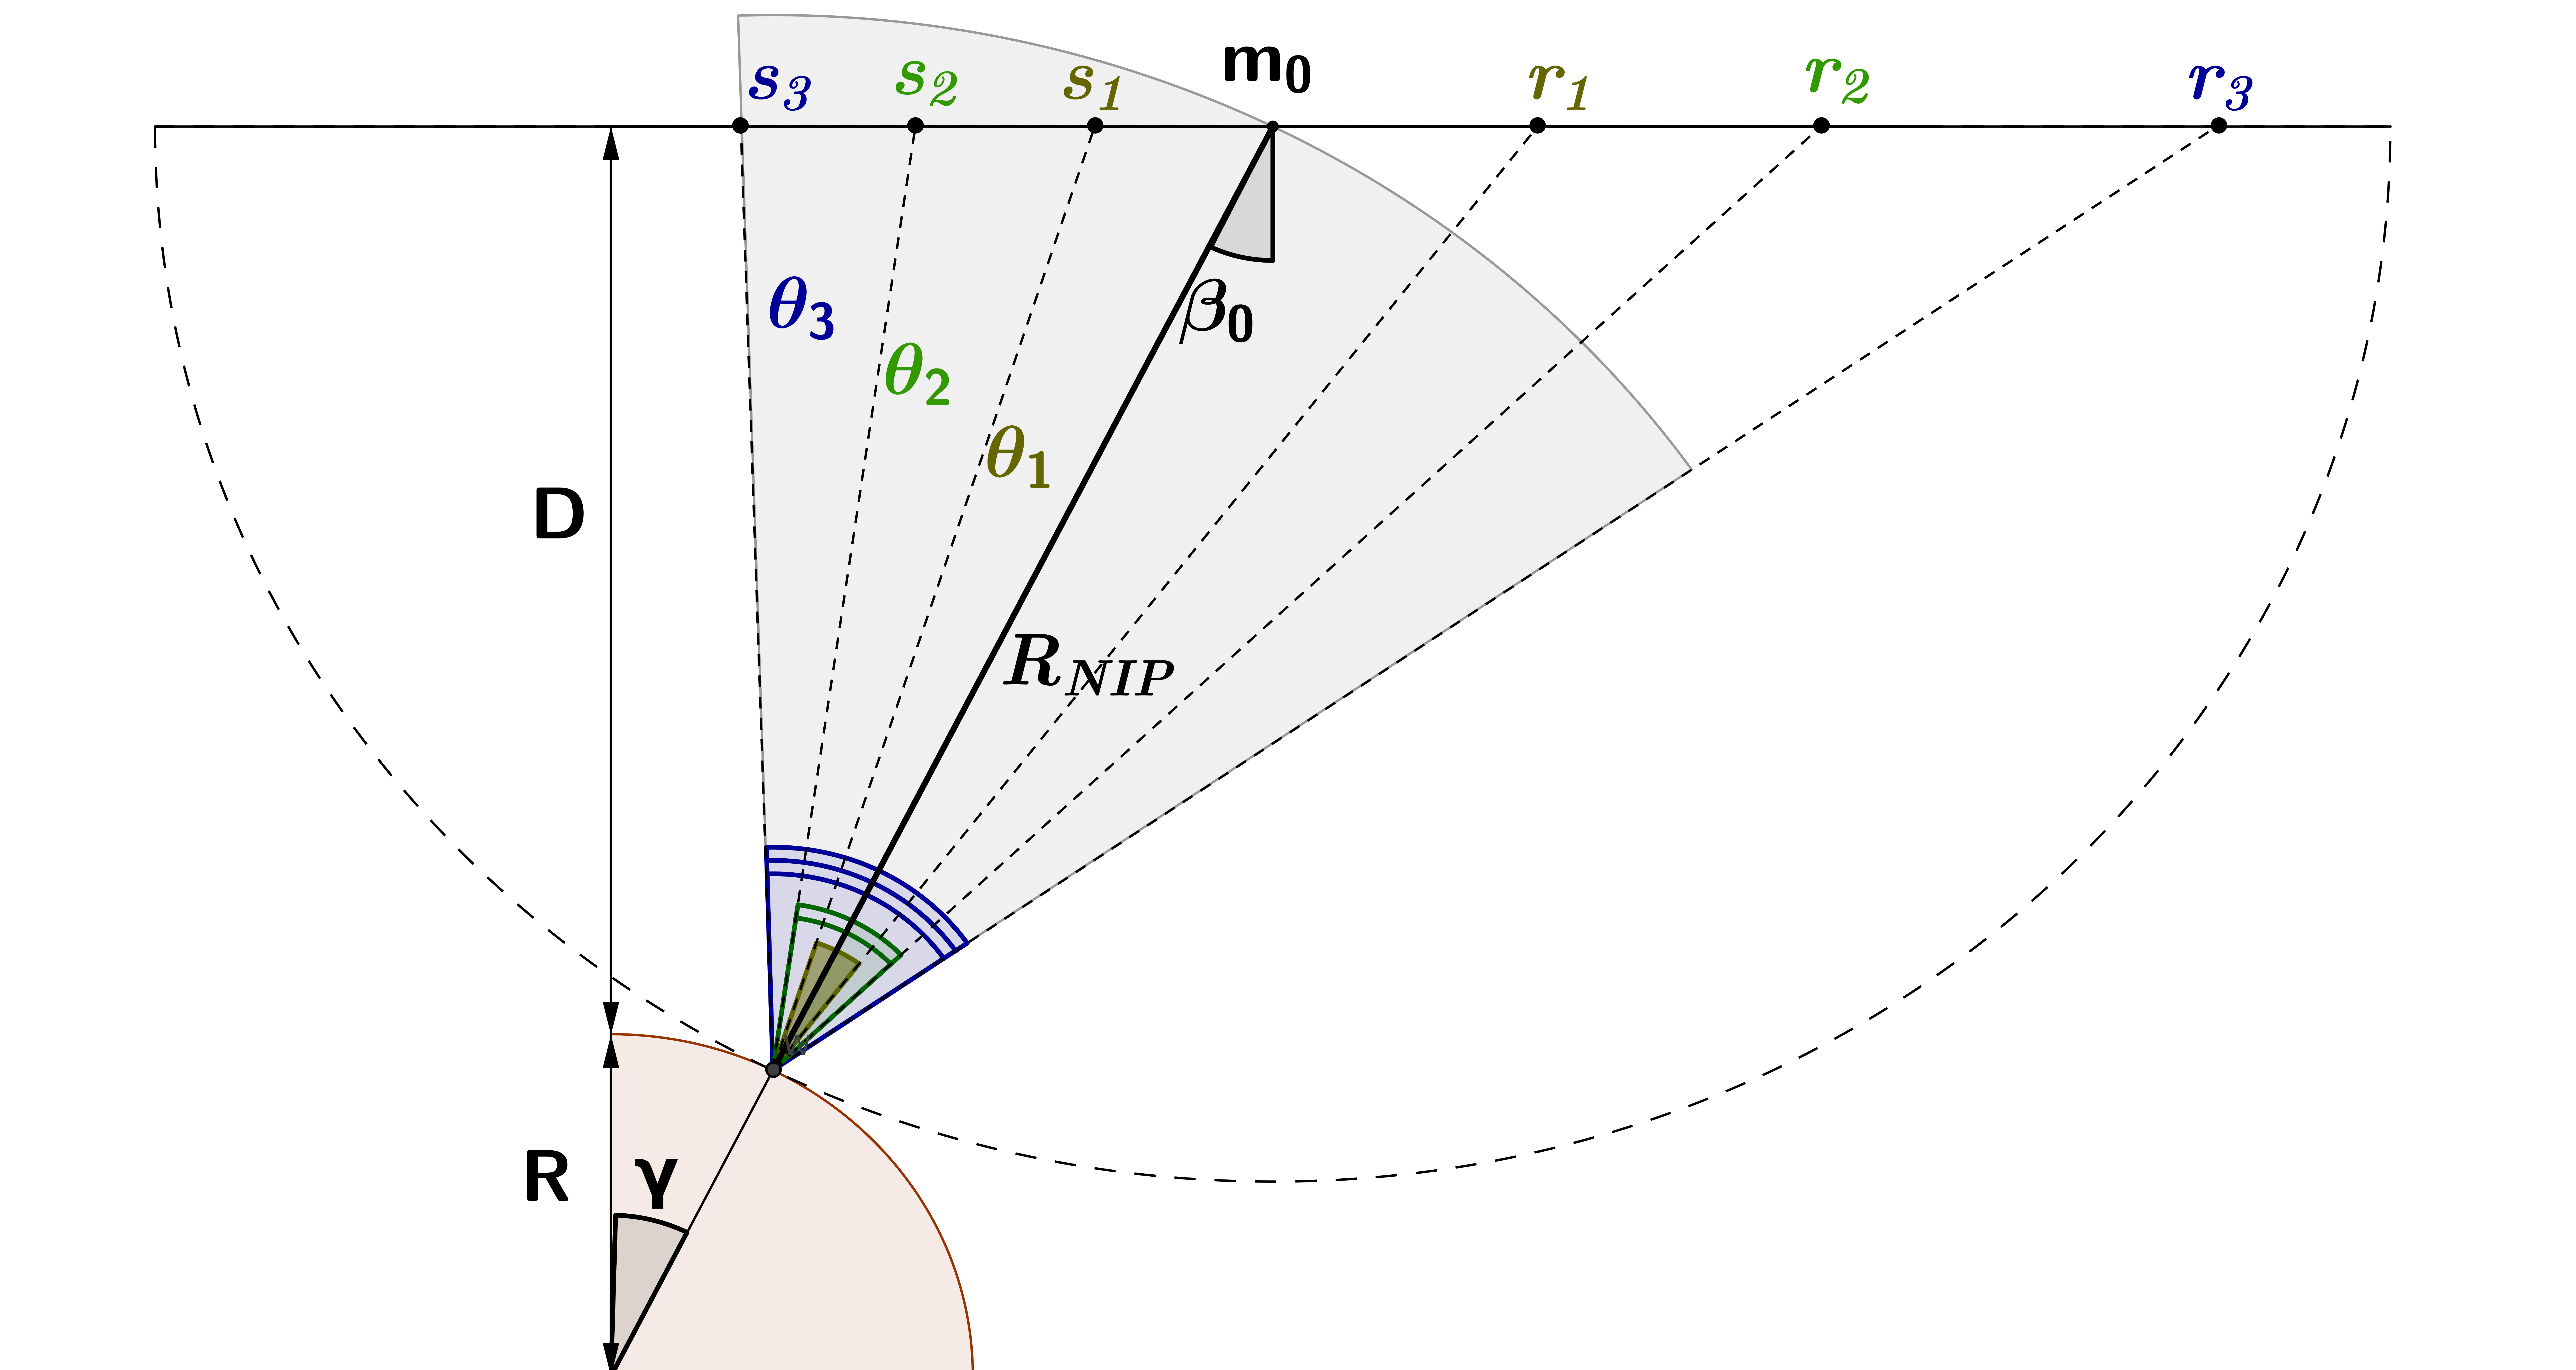
\includegraphics[scale=0.3]{images/cre.png}
\vspace{-0.3cm}
\end{center}
\begin{center}
 Fonte: Do Autor.
\end{center}
\label{fig:2.1}
\end{figure}

O principal desvantagem do método ERC é que as coordenadas de fontes e receptores são distribuídas assimetricamente em tal 
arranjo: Na Figura \ref{fig:2.1} representamos um arranjo ERC em um modelo do refletor circular 
em um meio com velocidade constante $v$.
Todos os raios de reflexão que saem das fontes $s_i$ e chegam aos receptores $r_i$ 
possuem o mesmo ponto de reflexão sobre o refletor.
Porém, a curvatura do refletor estabelece uma distribuição assimétrica dos pares fonte e receptor no domínio do afastamento $h$
e na distância em relação ao PMC central $m_0$, dada por $d=m-m_0$.

A Figura \ref{fig:2.2} mostra as coordenadas $m, h$ de várias curvas ERC hipotéticas com $\alpha$ dado pela Equação \ref{eq:2.2}.
As curvas ERC intersectam as seções de afastamento constante (linhas horizontais na figura) e as seções de ponto médio comum 
(linhas verticais na figura), não sendo posível construir uma malha regular para amostrar tais curvas simultaneamente nos dois
eixos.
A única distribuição que pode ser amostrada regularmente no plano $m, h$ ocorre quando $\alpha=0$. Esta é
a família de ponto médio comum do PMC $m_0$ (linha vertical com pontos em roxo na figura).

A Figura \ref{fig:2.2} mostra as coordenadas $m,h$ de várias curvas ERC hipotéticas com $\alpha$ dado pela Equação \ref{eq:2.2}.
As curvas ERC intersectam as seções de afastamento constante (linhas horizontais) e as seções de ponto médio comum 
(linhas verticais), não sendo posível construir uma malha regular para amostrar tais curvas.
A única distribuição que pode ser amostrada regularmente no plano $m,h$ ocorre quando $\alpha=0$, que corresponderá
a família de ponto médio comum de um dado $m_0$, uma linha vertical no plano (em roxo).

\begin{figure}[htb]
\caption{Representação esquemática das coordenadas de várias trajetórias ERC sobre o plano PMC $m$ x meio afastamento
$h$. As linhas do grid representam as seções de afastamento constante (linhas horizontais) e seções PMC (linhas verticais).
Estas trajetórias foram construídas variando $\beta_0$, $R_{NIP}$ e $\alpha$  na Equação \ref{eq:2.2}. Quando
$\alpha=0$ a trajetória ERC será a trajetória de uma família PMC para um PMC $m_0$.}
\begin{center}
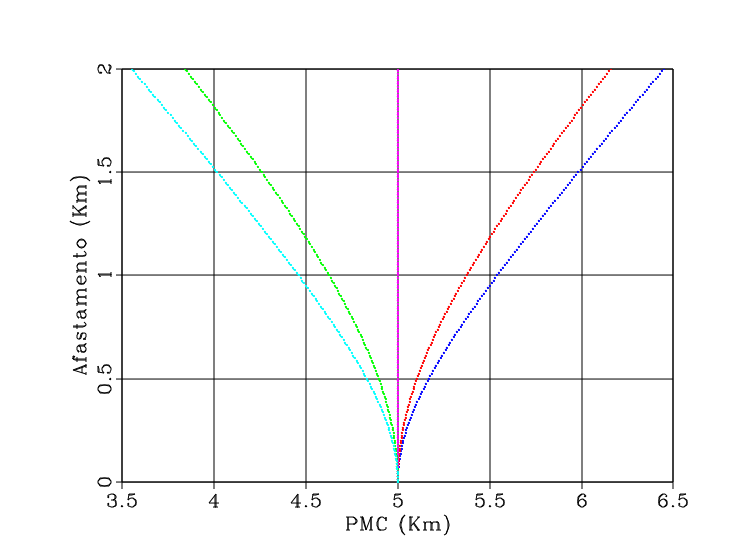
\includegraphics[scale=0.5]{images/creCoord.png}
\vspace{-0.3cm}
\end{center}
\begin{center}
 Fonte: Do Autor.
\end{center}
\label{fig:2.2}
\end{figure}

Neste trabalho propomos uma forma de aumentar a região de convergência da Equação \ref{eq:2.3} utilizando a
aproximação de tempo de trânsito do SRC não hiperbólico e aplicando a condição SDC ($R_N=R_{NIP}$) para
simular a trajetória de tempo de trânsito ERC: No modelo de uma fonte pontual sobre o refletor, o raio de 
curvatura $R_N$ é aproximadamente igual a $R_{NIP}$, esta condição limite é a condição SDC \cite{shav}.

Nossa hipótese é que ao utilizarmos a condição SDC na aproximação de tempo de trânsito do SRC não hiperbólico
teremos uma trajetória de tempo de trânsito ERC com uma região de convergência superior à Equação de tempo de
trânsito ERC (Equação \ref{eq:2.3}).

A aproximação do SRC não hiperbólico possui o
intuito de melhorar a acurácia das aproximações de tempo de trânsito SRC
para grandes afastamentos e separação entre os PMC's \cite{fomel1}.

\begin{equation}
\label{eq:2.4}
 \Phi_{CRS}(h,d;t_0)=\sqrt{\frac{F(d)+ch^2+\sqrt{F(d-h)F(d+h)}}{2}}
\end{equation}

A Equação \ref{eq:2.4} é chamada equação do CRS não-hiperbólico, pois não deriva de uma expansão em série de Taylor
de segunda ordem do tempo de trânsito. Os parâmetros 
$a_1$, $a_2$ e $b_2$
do CRS hiperbólico são utilizados na definição
dos parâmetros do SRC não hiperbólico como \cite{fomel1}:

\begin{equation}
\label{eq:2.5}
 c=2b_2+a_1^2-a_2
\end{equation}

\begin{equation}
\label{eq:2.6}
 F(d-h)=(t_0+a_1(d-h))^2+a_2(d-h)^2
\end{equation}

\begin{equation}
\label{eq:2.7}
 F(d+h)=(t_0+a_1(d+h))^2+a_2(d+h)^2
\end{equation} % Método CRE fundamentos teóricos
% \chapter{INTRODUÇÃO}
\label{cap1}

A equação do sobretempo normal \cite{dix} é uma aproximação de tempo de trânsito de reflexão válida para pequenos afastamentos
entre os pares fonte receptor na superfície de registro em uma aquisição sísmica. Esta equação foi desenvolvida para modelos de
multicamadas planas horizontais. 
A equação de sobretempo normal é uma aproximação em série de Taylor de segunda ordem para o tempo de trânsito, por isto é
também chamada de aproximação hiperbólica. Todavia, esta aproximação diverge do tempo de trânsito analítico
em grandes afastamentos.

Aproximações de tempo de trânsito não hiperbólicas foram desenvolvidas na literatura,
com o intuito de estender a região de convergência das
aproximações de tempo de trânsito no domínio do afastamento: Estas aproximações utilizam mais de dois termos para aumentar a 
acurácia da análise de velocidades e da correção de sobretempo normal. Cada uma destas aproximações terá
as suas limitações na estimativa das velocidades e na relação afastamento profundidade.

O empilhamento convencional, utilizando as aproximações de sobretempo normal hiperbólicas ou não hiperbólicas, é estendido
para o domínio do Ponto Médio Comun (PMC) a partir do empilhamento Superfície de Reflexão Comum (SRC) de
afastamento nulo: 
O empilhamento é realizado sobre uma superfície de tempo de
trânsito no domínio do meio afastamento $h$ e na vizinhança de um PMC central $m_0$, a partir de
três parâmetros ($R_N$, $R_{NIP}$ e $\beta_0$) dados para cada $m_0$. Este empilhamento SRC é dito de afastamento nulo,
pois o PMC central $m_0$ é escolhido da seção de afastamento nulo $h=0$.
O empilhamento SRC de afastamento nulo possui uma aproximação de tempo de trânsito hiperbólica \cite{jager},
e várias aproximações
de tempo de trânsito SRC foram propostas com o objetivo de estender a região de convergência desta aproximação:
As aproximações do SRC não hiperbólico \cite{fomel1}, as aproximações do SRC quarta ordem
\cite{germam}.

Um caso especial do método de empilhamento SRC, é o empilhamento por Elemento de Reflexão Comum (ERC):
O empilhamento ERC é também realizado no domínio do afastamento $h$ e na vizinhança de um PMC central $m_0$, assim como o
empilhamento SRC. Porém, o empilhamento ERC é feito sobre uma curva de tempo de trânsito de reflexão correspondente ao
conjunto de trajetórias de reflexão que possuem em comun
o mesmo ponto de incidência sobre o refletor.
Este método possui a vantagem de prover
parâmetros importantes para a construção do modelo de velocidades, e utiliza dois dos parâmetros
do método SRC de afastamento nulo ($R_{NIP}$ e $\beta_0$).
A principal desvantagem do método ERC é a interpolação: O empilhamento ERC necessita de 
traços em coordenadas de PMC $m$ e meio afastamento $h$ não coincidentes com as coordenadas
e amostragem dos dados adquiridos.
O objetivo desta pesquisa é propor uma metodologia de inversão do modelo de velocidades utilizando o método ERC para
a obtenção da seção empilhada e de interpolação dos dados observados para possibilitar a amostragem das famílias ERC. 

Propomos a seguinte estratégia de interpolação para a obtenção da seção empilhada ERC:
O algoritmo Very Fast Simulated Aneeling (VFSA) é utilizado para obter os parâmetros do SRC de afastamentos nulo
$R_{NIP}$ e $\beta_0$. Como a obtenção de tais parâmetros é um subproduto do empilhamento SRC esta etapa é comum
aos dois métodos, possibilitanto que os dois sejam realizados em fluxos de trabalho independentes que compartilham os 
mesmos parâmetros, não sendo necessário nenhum procedimento além do usual para o empilhamento SRC convencional.
A trajetória ERC é traçada no plano $m, h$ para estabelecer as coordenadas dos traços pertencentes à família ERC
com uma equação que descreve a trajetória e o a equação de tempo de trânsito ERC \cite{cre}.
Interpolaremos os dados adiquiridos utilizando os filtros adaptativos de predição de erro (FPE) no domínio PMC \cite{liu11}.
Esta etapa possibilita a amostragem adequada para a obtenção das famílias ERC,
uma para cada PMC central $m_0$. 
Finalizadas estas etapas,
obteremos a seção empilhada ERC a partir do empilhamento das amostras sobre uma curva de tempo de trânsito ERC 
pertencentes as famílias ERC. Esta curva é determinada para cadar par $m_0, t_0$ da seção empilhada \cite{cre}.

A principal vantagem do método ERC é não precisar de informação a priori do macromodelo de velocidades. 
Este método poder ser utilizado na obtenção do modelo de velocidades através de alguma etapa de inversão,
como a tomografia \cite{cre}. Para a obtenção do modelo de velocidades propomos a seguinte estratégia:
Utilização de um algoritmo iterativo iniciando com um modelo de velocidades inicial que é atualizado
a cada iteração com o algoritmo VFSA. 
O critério de convergência do modelo de velocidades será a coerência entre
os dados modelados a partir do modelo de velocidades da iteração atual com os dados pré empilhados \cite{mesquita}.

O modelo de velocidades de cada iteração do algoritmo de inversão será produzido a partir de respostas simuladas
de difrações em pontos $m_0, t_0$ escolhidos da seção empilhada ERC com uma equação de tempo de trânsito de difrações
e o espalhamento da amplitude do ponto escolhido $A(m_0, t_0)$ sobre a trajetória de tempo de trânsito, formando
a hipérbole de difração \cite{diffractions}. A focalização das difrações na seção empilhada ERC será realizada
através de um algoritmo baseado na continuação de velocidades e na medida de variação máxima local para produzir
os painéis de focalização da imagem com as velocidades que melhor focalizam as respostas de difrações simuladas.
Com o \textit{picking} das velocidades nestes painéis (máximos valores de variação máxima local indicam alta focalização)
é formado o modelo de velocidades da iteração atual \cite{sep_dif}.




 %INTRODUÇÃO
% \include{objetivo} % OBJETIVOS 1
% \include{justificativa} % 2
% \include{estado} % Estado da arte do problema 3
% \include{metodologia} % 4
% \include{resultados} % 5
% \chapter{CRONOGRAMA}
\label{cap9:cronograma}


\section{Etapas concluídas}

A seguir a descrição das etapas concluídas e o cronograma:

  \begin{enumerate}
   \item  Pesquisa e fundamentação teórica: Pesquisa das principais referências e estabelecimento do tema central da tese.
   \item   Modelagem Kirchhoff: Utilização do algoritmo de modelagem do pacote Madagascar\footnote{Madagascar é um pacote
   de procesamento sísmico 'open source' disponível em \url{http://www.ahay.org/wiki/Main_Page}.}
   \textit{sfkirmod} para produzir os dados do modelo do refletor
   gaussiano.
    \item Obtenção dos parâmetros do SRC utilizando o VFSA: Programa \textit{sfvfsacrenh} escrito  pelo Autor
    em linguagem C e adaptado para o pacote Madagascar
   baseado no algoritmo Very Fast Simulated Aneeling \cite{ingber}. O algoritmo ajusta a superfície de tempo de trânsito
   do SRC não hiperbólico (Equação \ref{eq:2.4}) aos dados modelados. Os parâmetros do SRC que produzem o melhor ajuste são
   os parâmetros otimizados.
    \item  Interpolação do cubo de dados com FPE: Interpolação das seções de afastamento constante extraídas dos dados modelados
    (chamado ``cubo de dados'') a partir de Filtros Adaptativos de Predição de Erro
    com os programas \textit{sfapef} e \textit{sfmiss4} do pacote Madagascar.
    Esta interpolação permite a discretização
    suficiente dos traços no domínio do PMC para possibilitar a correta amostragem das famílias ERC.
    \item  Cálculo das trajetórias ERC: Programa \textit{sfcretrajec} desenvolvido pelo Autor em linguagem C 
    e adaptado para o pacote Madagascar para
    o cálculo das trajetorias ERC baseado na Equação \ref{eq:2.1}.
     \item Obtenção das famílias ERC: Programa \textit{sfgetcregather} desenvolvido pelo Autor em linguagem C 
     e adaptado para o pacote Madagascar para a
     determinação dos traços sísmicos do cubo de dados que estão sobre as trajetorias ERC previamente calculadas na etapa anterior.
     Estes traços formam as famílias ERC.
    \item  Cálculo das curvas de empilhamento ERC: Programa \textit{sfgetcretimecurve} desenvolvido pelo Autor 
    em linguagem C e adaptado 
    para o pacote Madagascar para a determinação das curvas de tempo de trânsito ERC com auxílio das 
    Equações \ref{eq:2.3}-\ref{eq:2.4}.
     \item Paralelização do algoritmo com scons: Utilização de técnicas de computação paralela para melhorar o desempenho
     dos algoritmos desenvolvidos. O pacote Madagascar permite a Paralelização dos processos realizados a partir da execução
     com o comando \textit{scons -j\#} onde '\#' representa o número de núcleos utilizados.
    \item  Empilhamento e seção empilhada ERC: Programa \textit{sfcrestack} desenvolvido pelo Autor em linguagem C e adaptado 
    para o pacote Madagascar para a obtenção da seção  empilhada ERC.
  \end{enumerate}

    \begin{table}[H]
      \caption{Cronograma de trabalho das etapas já consluídas.}
      \centering
      
      \begin{tabular}{|c|c|c|}

      \hline
      \textbf{Etapas concluídas} & 2 & 3 \\ \hline
      Pesquisa e fundamentação teórica & x & x \\ \hline
      Modelagem Kirchhoff & x & x \\ \hline
      Obtenção dos parâmetros do SRC utilizando o VFSA & x & x \\ \hline
      Interpolação do cubo de dados com FPE & x & x \\ \hline
      Cálculo das trajetórias ERC & x & x \\ \hline
      Obtenção das famílias ERC & x & x \\ \hline
      Cálculo das curvas de empilhamento ERC & x & x \\ \hline
      Paralelização do algoritmo com scons & x & x \\ \hline
      Empilhamento e seção empilhada ERC & x & x  \\
      \hline
      
      \end{tabular}
  \end{table}
  
\section{Etapas ainda não concluídas}

A seguir a descrição das atividades ainda não realizadas e o cronograma:

  \begin{enumerate}
   \item Qualificação da tese
   \item Inversão do modelo de velocidades
   \item Defesa de tese
  \end{enumerate}
  
   \begin{table}[H]
      \caption{Cronograma de trabalho até o prazo final da defesa de tese.}
      \centering
      
      \begin{tabular}{|c|c|c|}

      \hline
      \textbf{Etapas ainda não concluídas} & 2 & 3 \\ \hline
      Qualificação da tese & x & x \\ \hline
      Inversão do modelo de velocidades & x & x \\ \hline
      Defesa de tese & x & x  \\
      \hline
      
      \end{tabular}
  \end{table}
  

Algumas observações: A data da apresentação para o Comitê de Avaliação de Tese é o dia 01 de Agosto de 2021.
A data da apresentação para a Banca Avaliadora dependerá das sugestões do
Comitê de Avaliação de Tese. A Previsão para defesa é entre os meses de Agosto de
2021 e Setembro de 2021.

 % 6
% \chapter{CONCLUSÃO}
\label{cap8:conclusao}
 %

\bookmarksetup{startatroot}

\bibliography{mybib}

%% Inicia os apêndices
%% ---
%\begin{apendicesenv}
%
%% Imprime uma página indicando o início dos apêndices
%\partapendices
%\newpage\null\thispagestyle{empty}
%\begin{center}
%\vspace{10cm}
%{\large\textbf{APÊNDICES}}
%\end{center}
%\newpage

% \input{apendiceA}
% \input{apendiceB}
% \input{apendiceC}
% \input{apendiceD}
% \input{MT}
%
%\end{apendicesenv}

%% Inicia os anexos
%\begin{anexosenv}
%\partanexos
%\include{AnexoA}

%\end{anexosenv}

\cleardoublepage
\phantomsection 
\printindex

\end{document}
